% Example figure showing segmentation with concrete array
\begin{figure}[t]
\centering
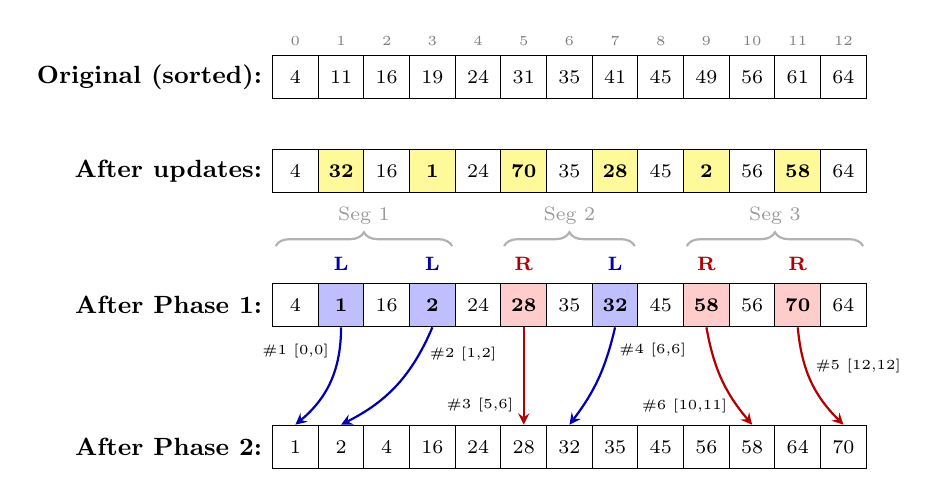
\begin{tikzpicture}[
    cell/.style={draw, minimum width=0.58cm, minimum height=0.55cm, font=\scriptsize},
    cellup/.style={cell, fill=yellow!40, font=\scriptsize\bfseries},
    cellL/.style={cell, fill=blue!25, font=\scriptsize\bfseries},
    cellR/.style={cell, fill=red!20, font=\scriptsize\bfseries},
    larrow/.style={->, >=stealth, thick, blue!70!black},
    rarrow/.style={->, >=stealth, thick, red!70!black},
    segbrace/.style={decorate, decoration={brace, amplitude=5pt}},
]

% === STAGE 1: Original sorted array ===
\node[font=\small\bfseries, anchor=east] at (-0.3, 0) {Original (sorted):};
\foreach \i/\v in {0/4, 1/11, 2/16, 3/19, 4/24, 5/31, 6/35, 7/41, 8/45, 9/49, 10/56, 11/61, 12/64} {
    \node[cell] (o\i) at (\i*0.58, 0) {\v};
}
% Index labels
\foreach \i in {0,...,12} {
    \node[font=\tiny, gray] at (\i*0.58, 0.45) {\i};
}

% === STAGE 2: After updates applied ===
\node[font=\small\bfseries, anchor=east] at (-0.3, -1.2) {After updates:};
\foreach \i/\v/\up in {0/4/0, 1/32/1, 2/16/0, 3/1/1, 4/24/0, 5/70/1, 6/35/0, 7/28/1, 8/45/0, 9/2/1, 10/56/0, 11/58/1, 12/64/0} {
    \ifnum\up=1
        \node[cellup] (u\i) at (\i*0.58, -1.2) {\v};
    \else
        \node[cell] (u\i) at (\i*0.58, -1.2) {\v};
    \fi
}

% === STAGE 3: After Phase 1 (sorted updates, L/R classified) ===
\node[font=\small\bfseries, anchor=east] at (-0.3, -2.9) {After Phase 1:};

% Segment braces (between Stage 2 and L/R labels)
\draw[segbrace, thick, gray!60] (0*0.58-0.25, -2.15) -- (3*0.58+0.25, -2.15) 
    node[midway, above=4pt, font=\scriptsize, gray!80] {Seg 1};
\draw[segbrace, thick, gray!60] (5*0.58-0.25, -2.15) -- (7*0.58+0.25, -2.15) 
    node[midway, above=4pt, font=\scriptsize, gray!80] {Seg 2};
\draw[segbrace, thick, gray!60] (9*0.58-0.25, -2.15) -- (12*0.58+0.25, -2.15) 
    node[midway, above=4pt, font=\scriptsize, gray!80] {Seg 3};

% L/R labels (just above Phase 1 array)
\node[font=\scriptsize, blue!70!black] at (1*0.58, -2.38) {\textbf{L}};
\node[font=\scriptsize, blue!70!black] at (3*0.58, -2.38) {\textbf{L}};
\node[font=\scriptsize, red!70!black] at (5*0.58, -2.38) {\textbf{R}};
\node[font=\scriptsize, blue!70!black] at (7*0.58, -2.38) {\textbf{L}};
\node[font=\scriptsize, red!70!black] at (9*0.58, -2.38) {\textbf{R}};
\node[font=\scriptsize, red!70!black] at (11*0.58, -2.38) {\textbf{R}};

% Phase 1 array: 4, 1, 16, 2, 24, 28, 35, 32, 45, 58, 56, 70, 64
% Only color violation cells (L=blue, R=red), others plain
\node[cell] (p0) at (0*0.58, -2.9) {4};
\node[cellL] (p1) at (1*0.58, -2.9) {1};
\node[cell] (p2) at (2*0.58, -2.9) {16};
\node[cellL] (p3) at (3*0.58, -2.9) {2};
\node[cell] (p4) at (4*0.58, -2.9) {24};
\node[cellR] (p5) at (5*0.58, -2.9) {28};
\node[cell] (p6) at (6*0.58, -2.9) {35};
\node[cellL] (p7) at (7*0.58, -2.9) {32};
\node[cell] (p8) at (8*0.58, -2.9) {45};
\node[cellR] (p9) at (9*0.58, -2.9) {58};
\node[cell] (p10) at (10*0.58, -2.9) {56};
\node[cellR] (p11) at (11*0.58, -2.9) {70};
\node[cell] (p12) at (12*0.58, -2.9) {64};

% === STAGE 4: After Phase 2 (fully sorted) ===
\node[font=\small\bfseries, anchor=east] at (-0.3, -4.7) {After Phase 2:};

% Final sorted: 1, 2, 4, 16, 24, 28, 32, 35, 45, 56, 58, 64, 70
\foreach \i/\v in {0/1, 1/2, 2/4, 3/16, 4/24, 5/28, 6/32, 7/35, 8/45, 9/56, 10/58, 11/64, 12/70} {
    \node[cell] (f\i) at (\i*0.58, -4.7) {\v};
}

% Movement arrows from Phase 1 to Phase 2 (updated values only)
% Labels show: #fix_number (leftBound, rightBound) - placed beside arrows
\draw[larrow, bend left=25] (p1.south) to node[font=\tiny, black, left, pos=0.2] {\#1 [0,0]} (f0.north);
\draw[larrow, bend left=20] (p3.south) to node[font=\tiny, black, right, pos=0.2] {\#2 [1,2]} (f1.north);
\draw[rarrow] (p5.south) to node[font=\tiny, black, left, pos=0.8] {\#3 [5,6]} (f5.north);
\draw[larrow, bend left=12] (p7.south) to node[font=\tiny, black, right, pos=0.2] {\#4 [6,6]} (f6.north);
\draw[rarrow, bend right=15] (p9.south) to node[font=\tiny, black, left, pos=0.8] {\#6 [10,11]} (f10.north);
\draw[rarrow, bend right=20] (p11.south) to node[font=\tiny, black, right, pos=0.35] {\#5 [12,12]} (f12.north);

\end{tikzpicture}
\caption{Segmentation example: An array of size 13 with 6 updates at indices 1, 3, 5, 7, 9, 11. 
In \textbf{Phase~1}, updated values are sorted among themselves and written back to the array. Each value is classified as \textcolor{blue!70!black}{L} or \textcolor{red!70!black}{R}.
In \textbf{Phase~2}, each value is fixed one by one. The label numbers indicate the fixing order, along with the computed left and right bounds for binary search for each updated value.}
\label{fig:delta-sort-example}
\end{figure}